\subsubsection{SIMD化}
SIMDとはSingle Instruction Multiple Dataの略のことであり, その名の通り一つの命令を複数のデータに対して同時に適用する命令のことを指す.\\
C言語においてSIMD命令は明示的にSIMDの利用を定義する方法( TODO: add desc)と, コンパイラによる自動的なSIMD化があるが,
本研究では後者のコンパイラによるSMID化を促進する手法のみを扱う.\\
$c = a + b$という式をSIMD命令を用いて実行すると図\ref{fig:simd-image}のようになるため,
コンパイラが自動的にSIMD化を行うためには演算対処のデータ構造がベクトル化されていることが必要となる.\\
\begin{figure}[h!]
% h:here, t:top, b:bottom, p:page
%  \begin{left}
%    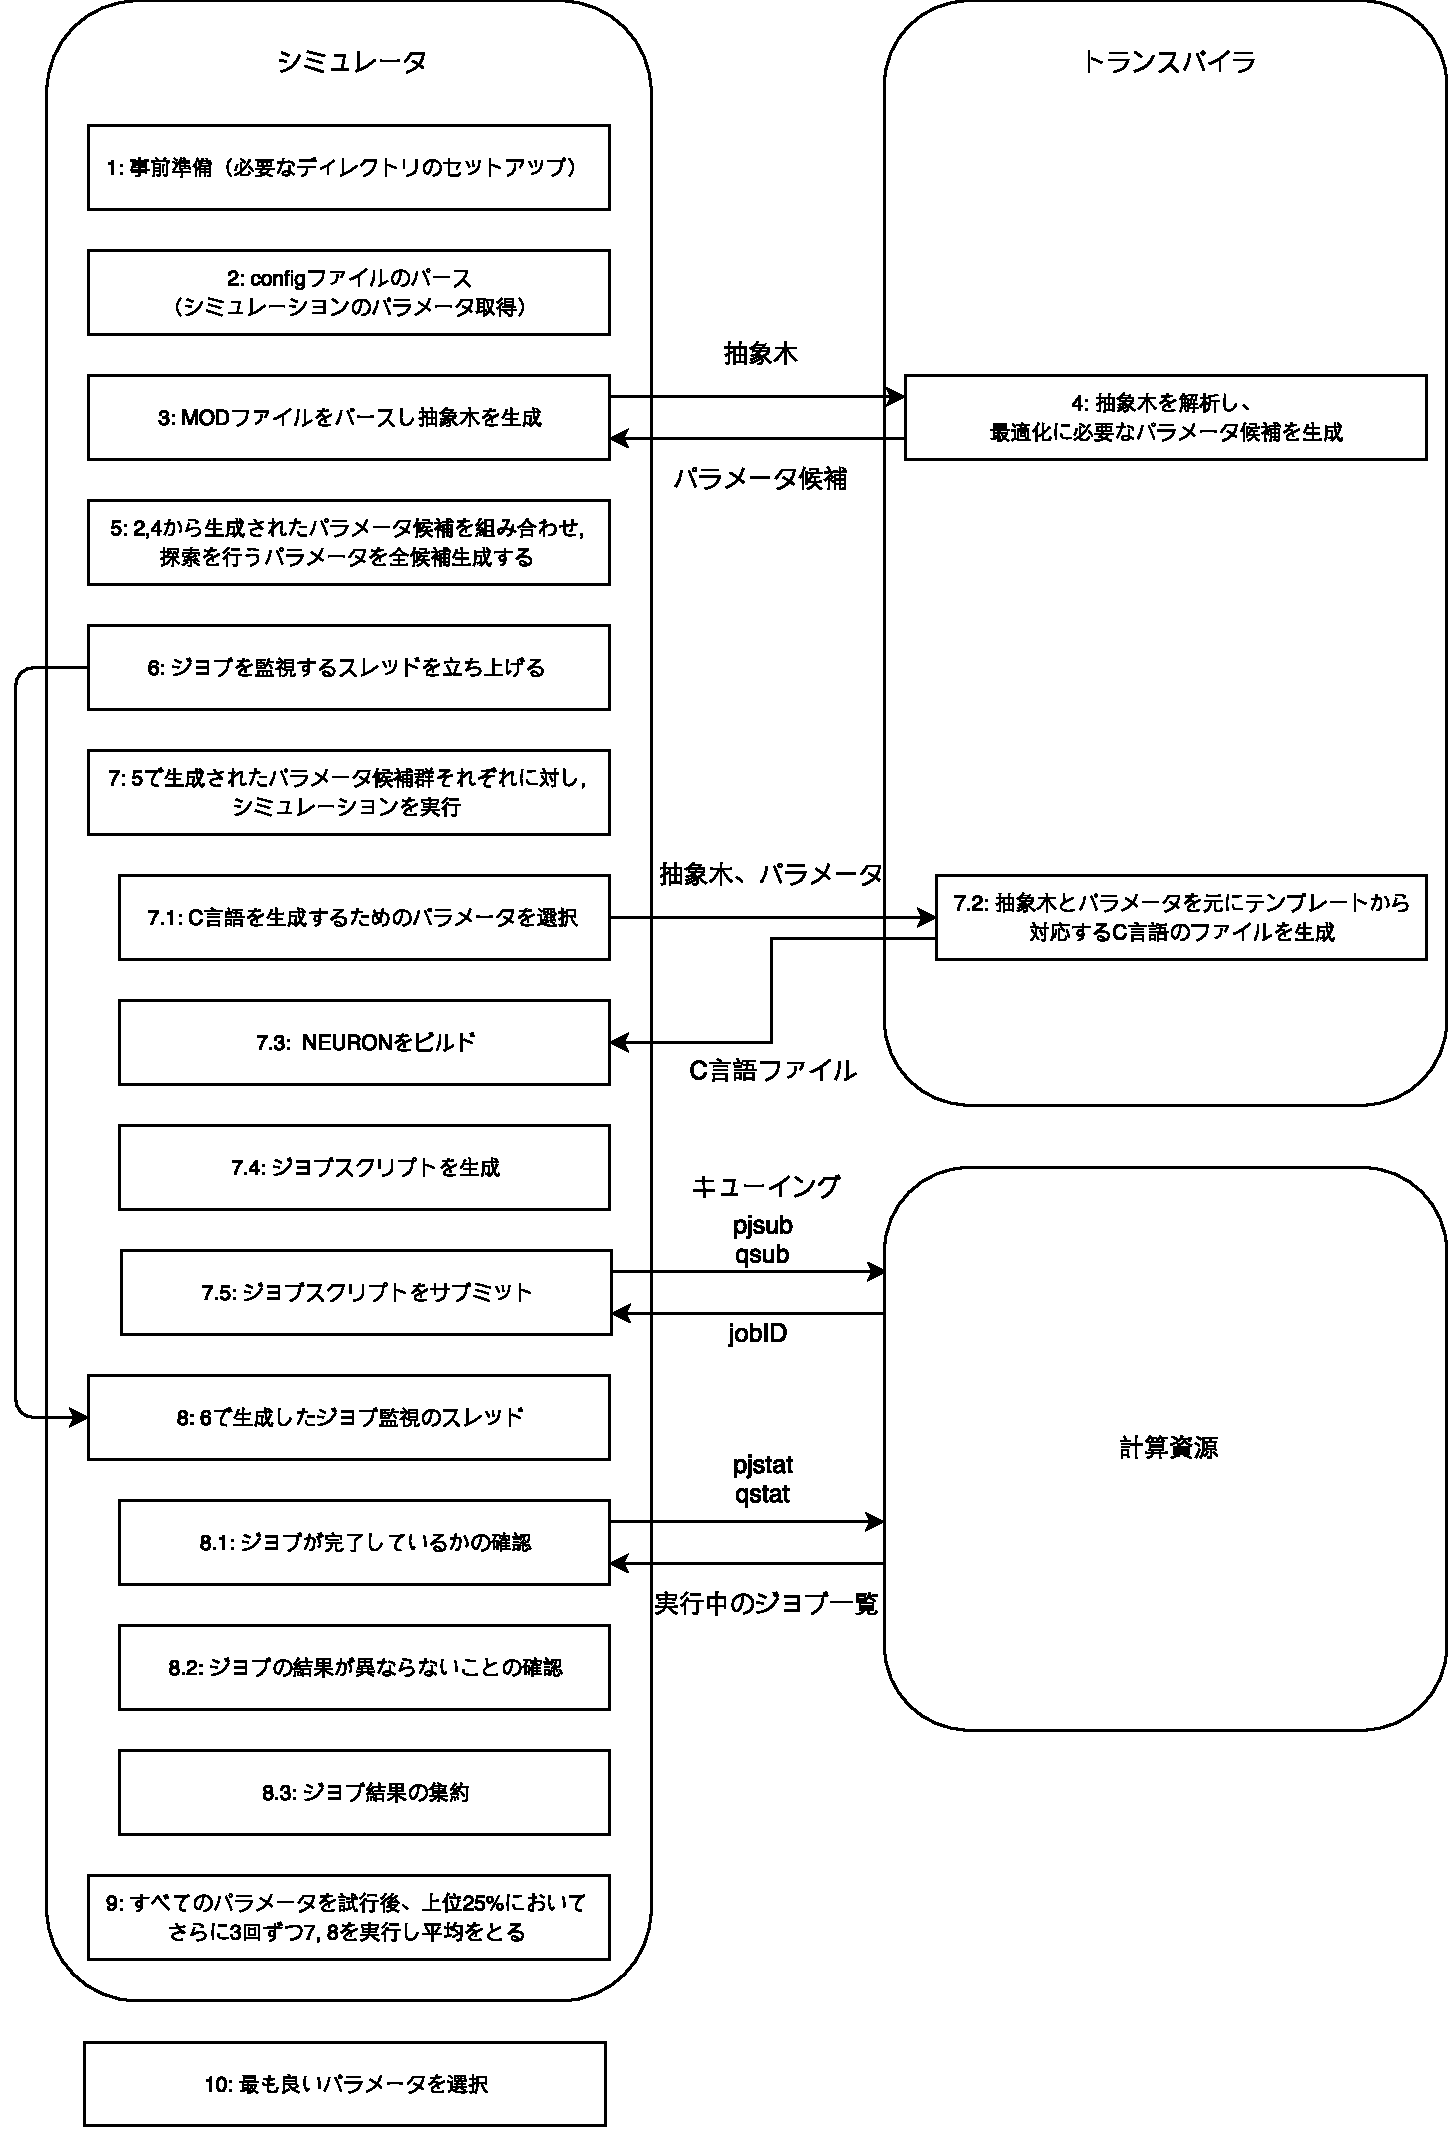
\includegraphics[width=18.0cm]{./images/Genie.pdf}
    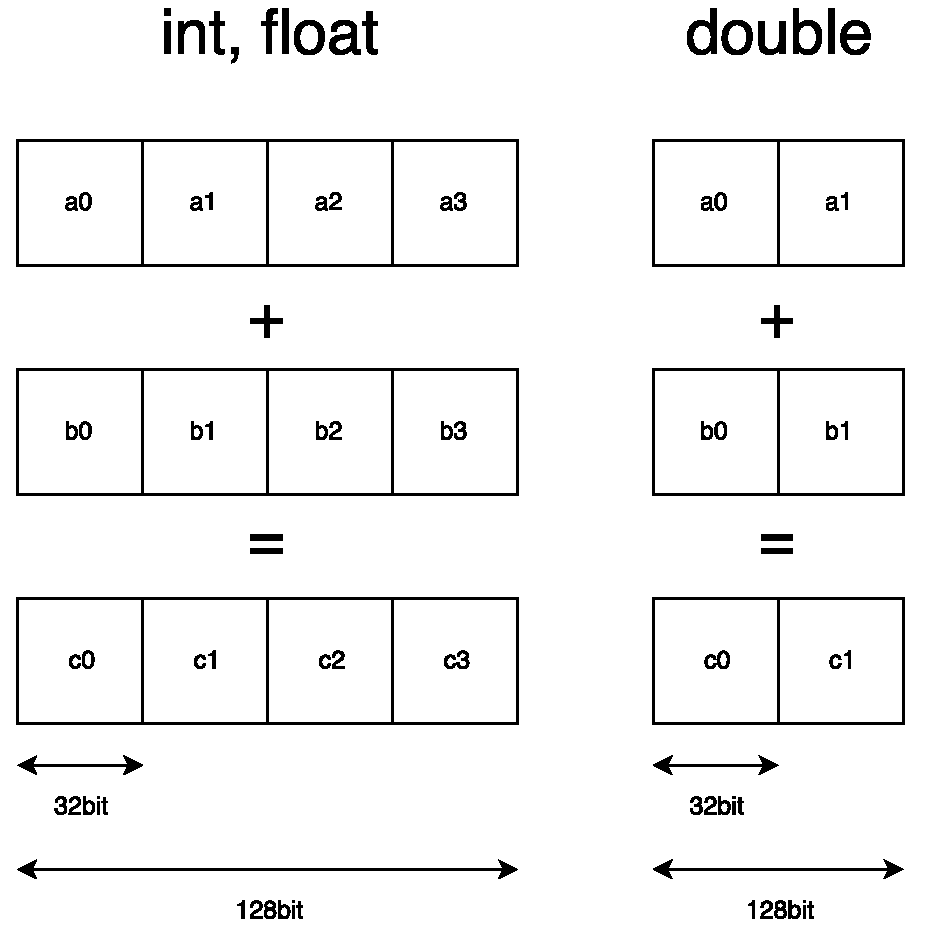
\includegraphics[width=1.1\textwidth]{./images/SIMD.pdf}
    \caption{SIMD命令}
    \label{fig:simd-image}
%  \end{left}
\end{figure}~\\

本研究で利用する計算機には双方ともこのSIMD命令を実行できるFMA (Fused Multiply Add)が搭載されており,
このFMAでは和の計算だけでなく積和演算を行うことができる.\\
\begin{figure}[h!]
% h:here, t:top, b:bottom, p:page
%  \begin{left}
%    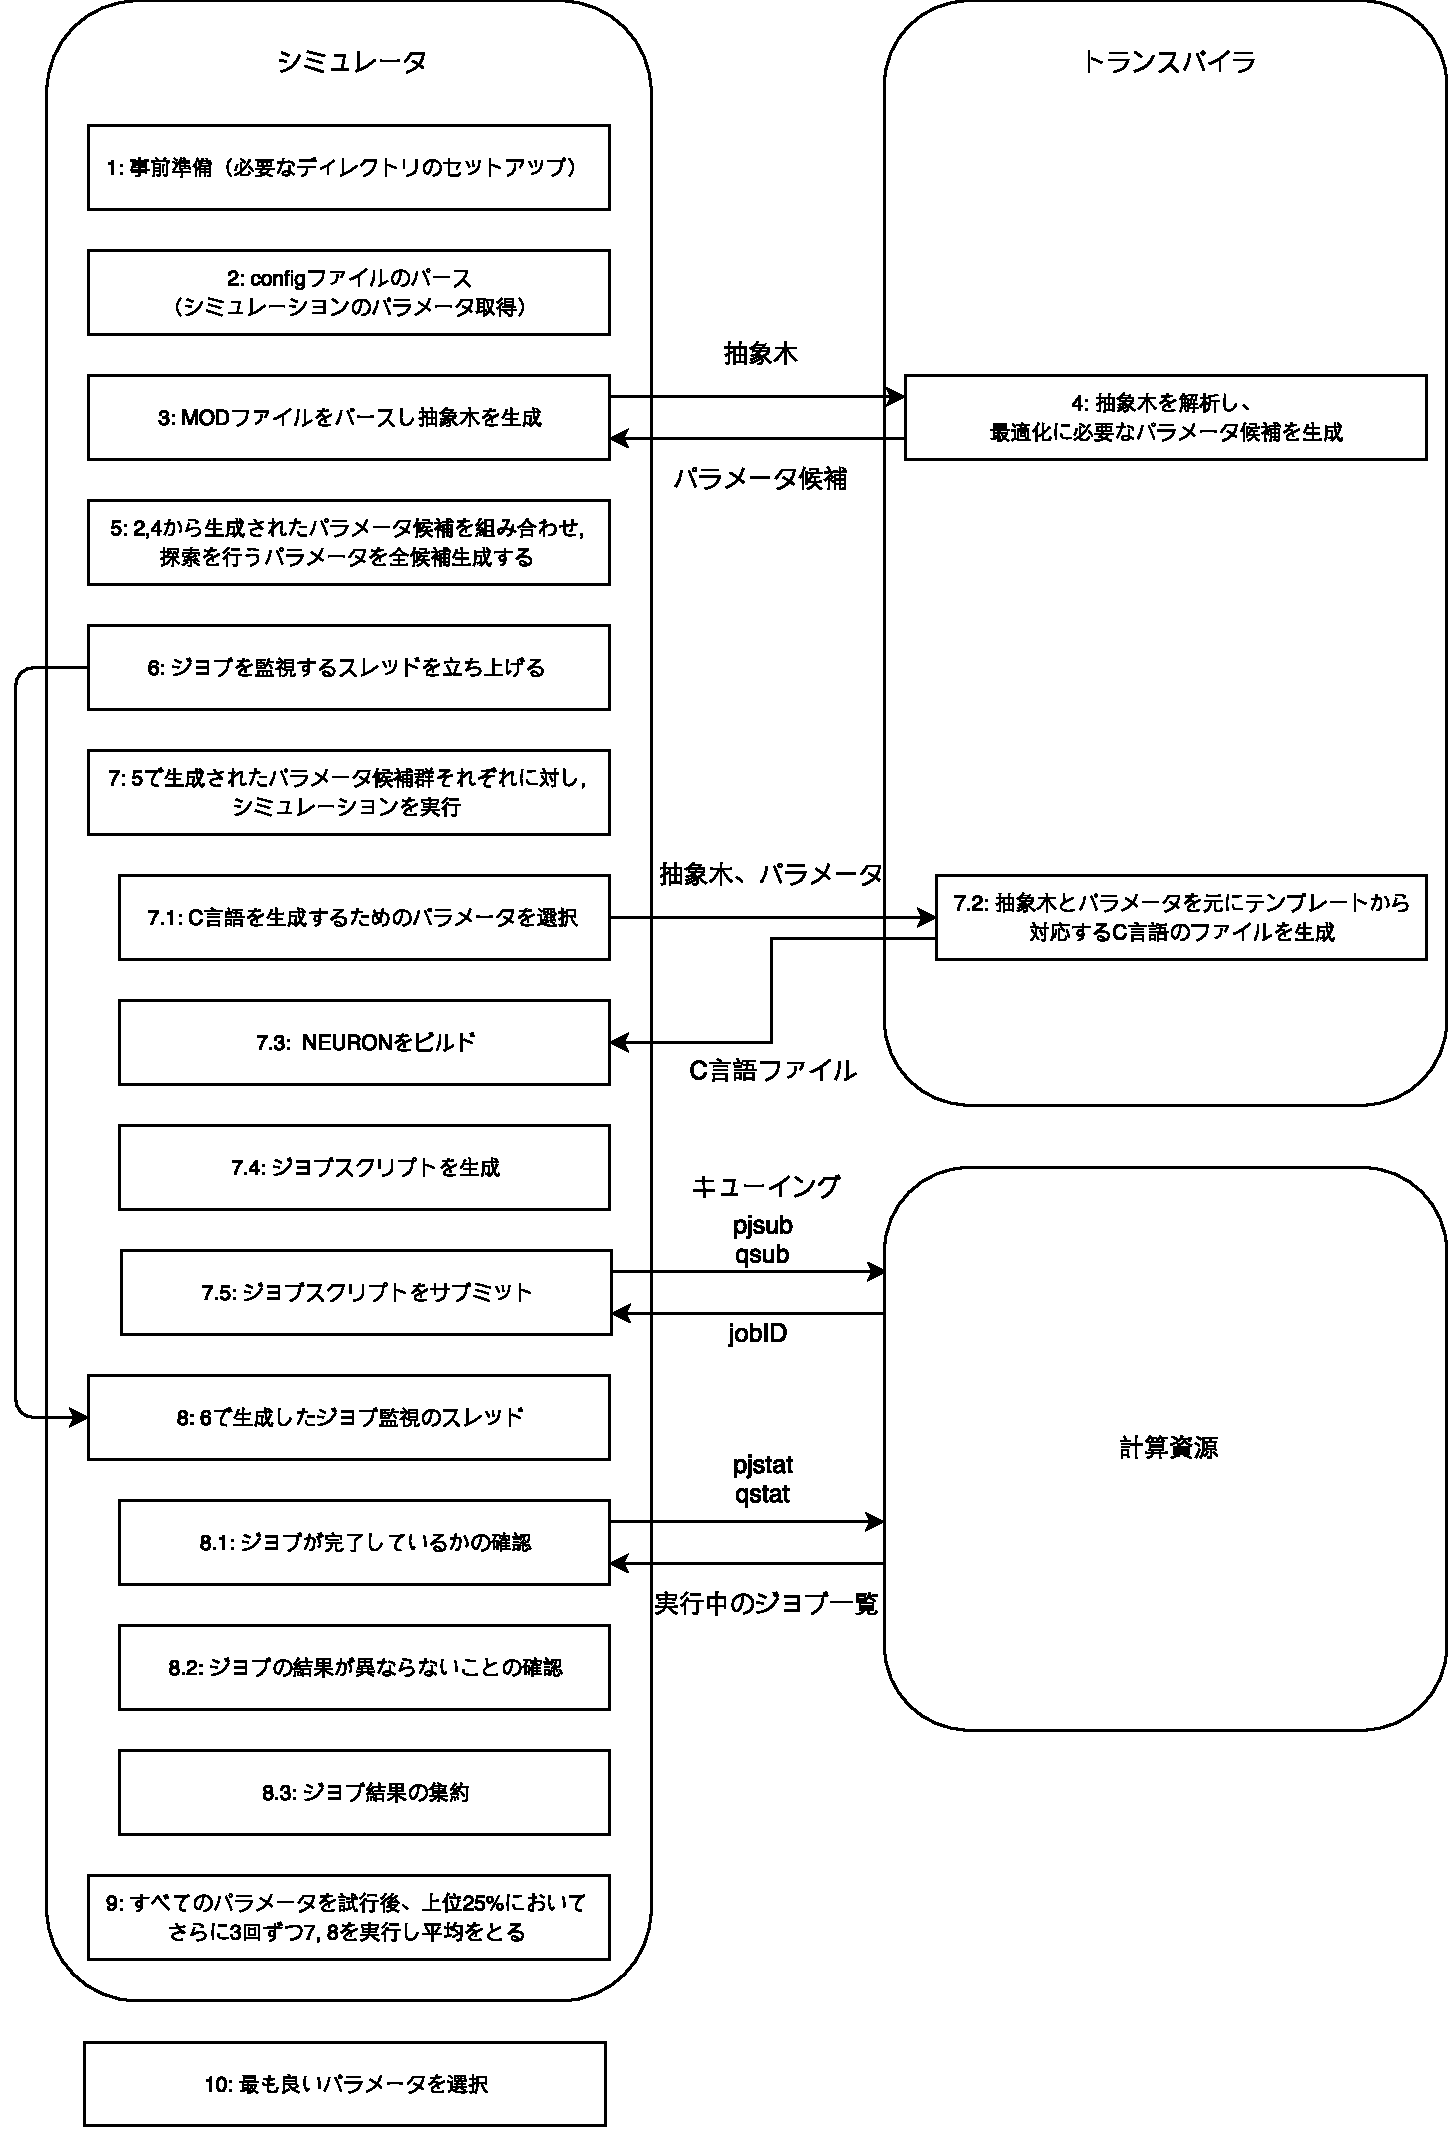
\includegraphics[width=18.0cm]{./images/Genie.pdf}
    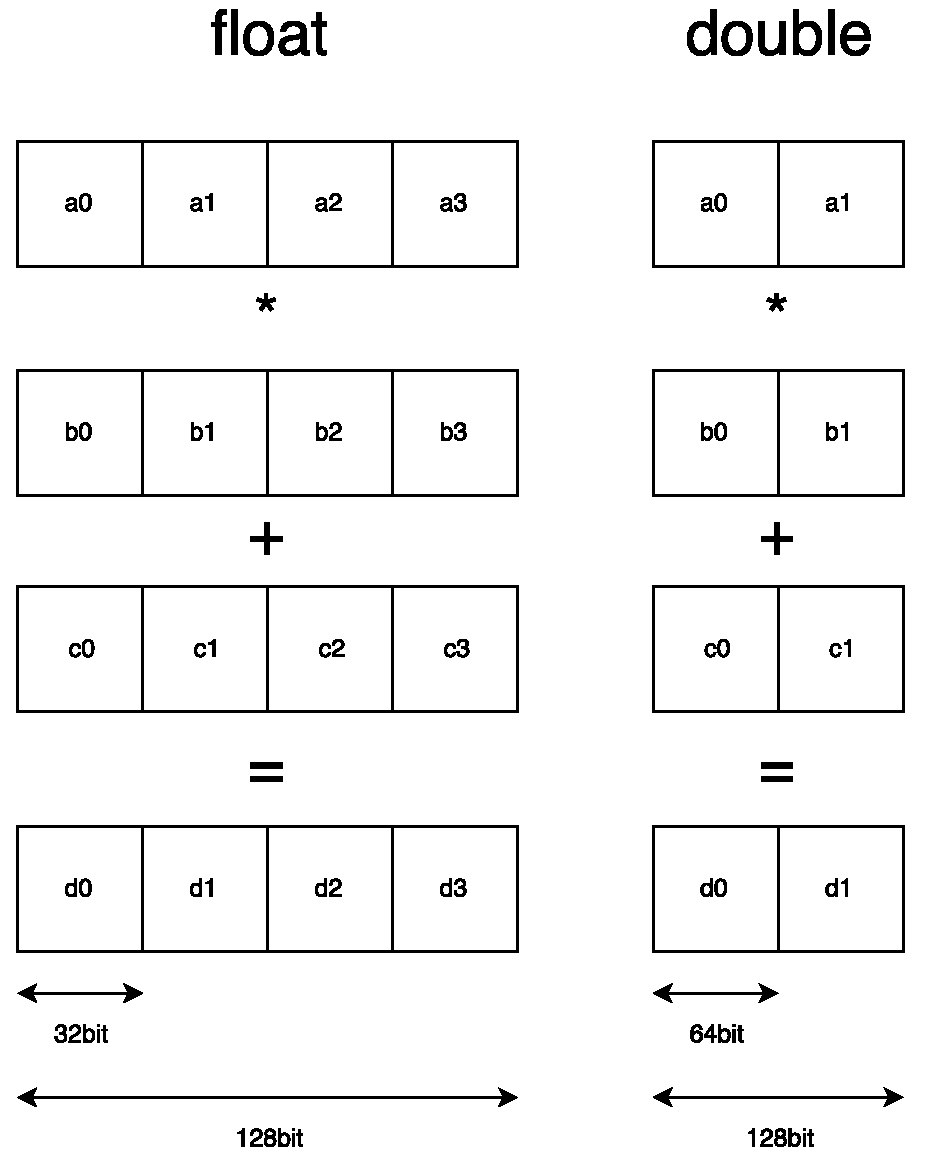
\includegraphics[width=1.1\textwidth]{./images/FMA.pdf}
    \caption{FMA}
    \label{fig:fma-image}
%  \end{left}
\end{figure}~\\

京についての計算性能の理論値は, \\
・1ノード = 8CPUコア\\
・クロック = 2GHz\\
・SIMD = 2 × FMA / core\\
となるため, SIMDを使わない場合は\\
・8 × 2 GFLOPS = 1 Floating-point Operation × 2 GHz × 8コア\\
SIMDを使う場合は\\
・8 × 16 GFLOPS = 4 Floating-point Operation × 2 SIMD Unit × 2GHz × 8コア\\
となり計算性能に大きな差が出る.\\

同様にクラスタにおいての計算性能は,\\
( TODO 値をちゃんとする)
・1ノード = 14CPUコア\\
・クロック = 2.4GHz\\
・SIMD = 2 × FMA / core\\
となるため, SIMDを使わない場合は\\
・14 × 2.4 GFLOPS = 1 Floating-point Operation × 2.4 GHz × 14コア\\
SIMDを使う場合は\\
・14 × 19.2 GFLOPS = 4 Floating-point Operation × 2 SIMD Unit × 2.4GHz × 14コア\\
となり計算性能に大きな差が出る.\\

以上から, SIMD命令を用いることができる環境においては, コンパイラによるSIMD化を促進することで大きな計算性能の向上が期待できるため
最適化の手法としてデータ構造の配列化は大きな意義を持つと考えられる.
